% C093: a=4, A=1, c=2; E: x^2/16+y^2/12=1, H: x^2-y^2/3=1
% Intersection P=(2,3); PF1=5, PF2=3; generated as exact coordinate constructions.
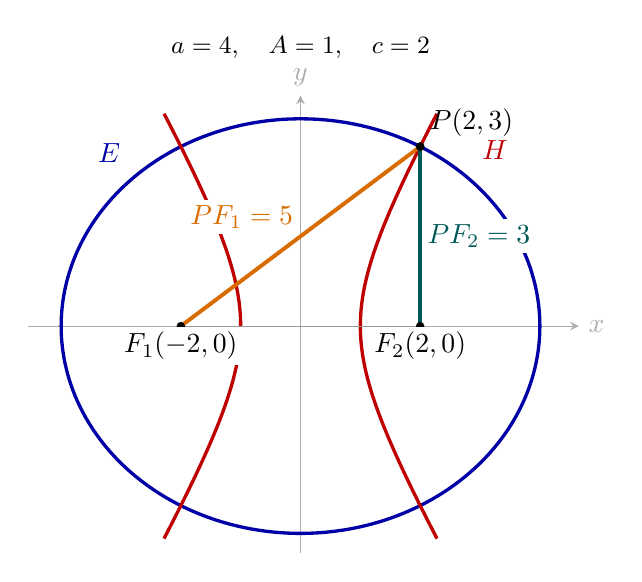
\begin{tikzpicture}[scale=0.76,>=stealth]
 \node[font=\small] at (0,4.65) {$a=4,\quad A=1,\quad c=2$};
 \draw[->,gray!65] (-4.55,0)--(4.65,0) node[right]{$x$};
 \draw[->,gray!65] (0,-3.8)--(0,3.85) node[above]{$y$};
 \draw[blue!65!black,very thick,samples=160,domain=0:360,smooth,variable=\t]
  plot ({4*cos(\t)},{sqrt(12)*sin(\t)});
 \draw[red!75!black,very thick,samples=110,domain=-3.55:3.55,variable=\t]
  plot ({sqrt(1+\t*\t/3)},{\t});
 \draw[red!75!black,very thick,samples=110,domain=-3.55:3.55,variable=\t]
  plot ({-sqrt(1+\t*\t/3)},{\t});
 \coordinate (L) at (-2,0); \coordinate (R) at (2,0); \coordinate (P) at (2,3);
 \draw[orange!85!black,line width=1.4pt] (L)--(P) node[midway,above left,fill=white,inner sep=2pt]{$PF_1=5$};
 \draw[teal!70!black,line width=1.4pt] (R)--(P) node[midway,right,fill=white,inner sep=2pt]{$PF_2=3$};
 \draw[gray!80] (L)--(R);
 \fill (L) circle (2pt) node[below,fill=white,inner sep=2pt]{$F_1(-2,0)$};
 \fill (R) circle (2pt) node[below,fill=white,inner sep=2pt]{$F_2(2,0)$};
 \fill (P) circle (2.1pt) node[above right]{$P(2,3)$};
 \node[blue!65!black] at (-3.2,2.9) {$E$};
 \node[red!75!black] at (3.25,2.95) {$H$};
\end{tikzpicture}
